% Généré par build/plot_ladders_main.py — ne pas éditer à la main.
% Source : results/main_ladders_n10000.json (seed 20260827, 10000 traj.).
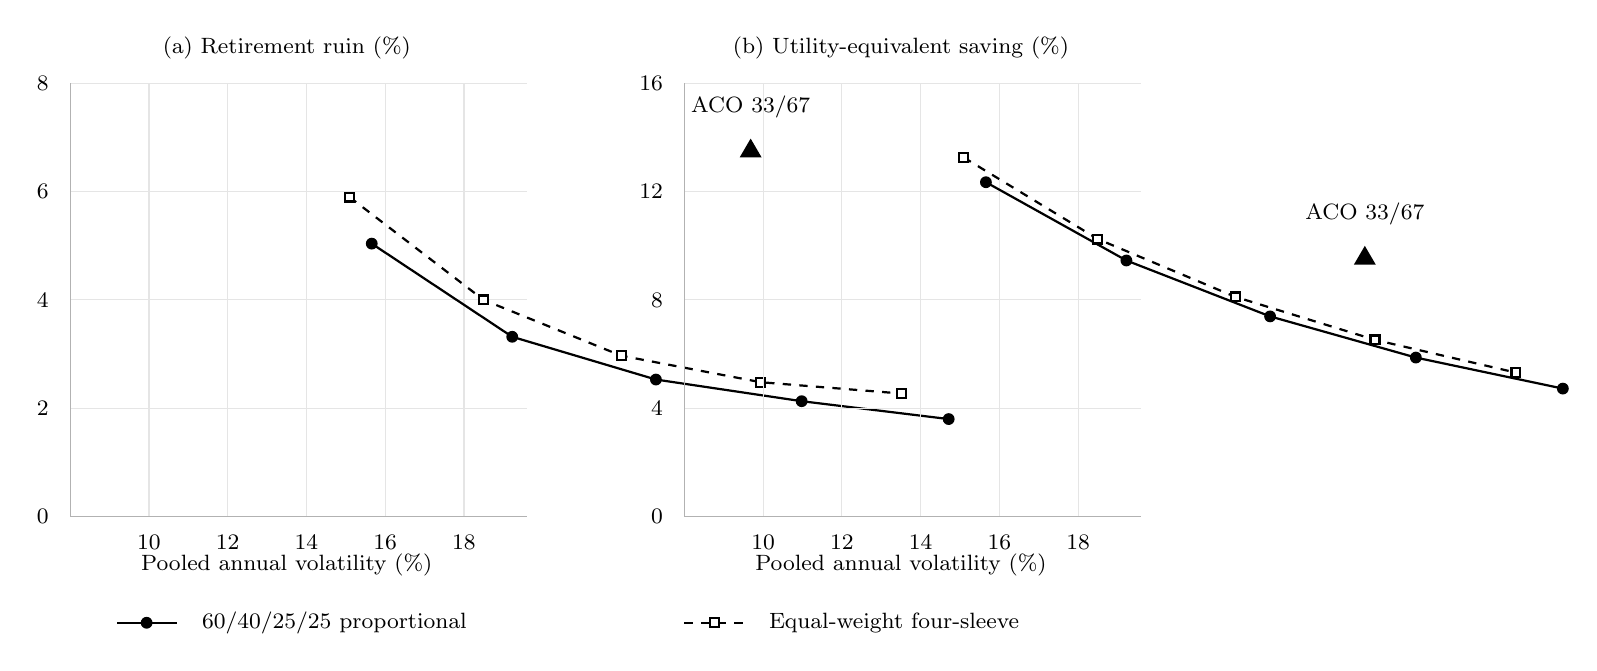
\begin{tikzpicture}[x=1cm, y=1cm]
\begin{scope}[shift={(0.0,0)}]
  \draw[gray!20] (0,0.000) -- (5.80,0.000);
  \node[left, font=\footnotesize] at (-0.15,0.000) {0};
  \draw[gray!20] (0,1.375) -- (5.80,1.375);
  \node[left, font=\footnotesize] at (-0.15,1.375) {2};
  \draw[gray!20] (0,2.750) -- (5.80,2.750);
  \node[left, font=\footnotesize] at (-0.15,2.750) {4};
  \draw[gray!20] (0,4.125) -- (5.80,4.125);
  \node[left, font=\footnotesize] at (-0.15,4.125) {6};
  \draw[gray!20] (0,5.500) -- (5.80,5.500);
  \node[left, font=\footnotesize] at (-0.15,5.500) {8};
  \draw[gray!20] (1.000,0) -- (1.000,5.500);
  \node[below, font=\footnotesize] at (1.000,-0.12) {10};
  \draw[gray!20] (2.000,0) -- (2.000,5.500);
  \node[below, font=\footnotesize] at (2.000,-0.12) {12};
  \draw[gray!20] (3.000,0) -- (3.000,5.500);
  \node[below, font=\footnotesize] at (3.000,-0.12) {14};
  \draw[gray!20] (4.000,0) -- (4.000,5.500);
  \node[below, font=\footnotesize] at (4.000,-0.12) {16};
  \draw[gray!20] (5.000,0) -- (5.000,5.500);
  \node[below, font=\footnotesize] at (5.000,-0.12) {18};
  \draw[gray!60] (0,0) -- (5.80,0);
  \draw[gray!60] (0,0) -- (0,5.500);
  \fill (8.641,4.799) -- ++(-0.14,-0.24) -- ++(0.28,0) -- cycle;
  \node[font=\footnotesize, anchor=south] at (8.641,4.939) {ACO 33/67};
  \draw[thick] plot coordinates {(3.829,3.465) (5.613,2.282) (7.438,1.739) (9.289,1.464) (11.156,1.237)};
  \fill (3.829,3.465) circle (0.075);
  \fill (5.613,2.282) circle (0.075);
  \fill (7.438,1.739) circle (0.075);
  \fill (9.289,1.464) circle (0.075);
  \fill (11.156,1.237) circle (0.075);
  \draw[thick, dashed] plot coordinates {(3.547,4.056) (5.250,2.750) (6.997,2.042) (8.770,1.705) (10.560,1.561)};
  \node[draw, thick, rectangle, inner sep=1.6pt, fill=white] at (3.547,4.056) {};
  \node[draw, thick, rectangle, inner sep=1.6pt, fill=white] at (5.250,2.750) {};
  \node[draw, thick, rectangle, inner sep=1.6pt, fill=white] at (6.997,2.042) {};
  \node[draw, thick, rectangle, inner sep=1.6pt, fill=white] at (8.770,1.705) {};
  \node[draw, thick, rectangle, inner sep=1.6pt, fill=white] at (10.560,1.561) {};
  \node[font=\footnotesize] at (2.75,5.95) {(a) Retirement ruin (\%)};
  \node[font=\footnotesize] at (2.75,-0.62) {Pooled annual volatility (\%)};
\end{scope}
\begin{scope}[shift={(7.8,0)}]
  \draw[gray!20] (0,0.000) -- (5.80,0.000);
  \node[left, font=\footnotesize] at (-0.15,0.000) {0};
  \draw[gray!20] (0,1.375) -- (5.80,1.375);
  \node[left, font=\footnotesize] at (-0.15,1.375) {4};
  \draw[gray!20] (0,2.750) -- (5.80,2.750);
  \node[left, font=\footnotesize] at (-0.15,2.750) {8};
  \draw[gray!20] (0,4.125) -- (5.80,4.125);
  \node[left, font=\footnotesize] at (-0.15,4.125) {12};
  \draw[gray!20] (0,5.500) -- (5.80,5.500);
  \node[left, font=\footnotesize] at (-0.15,5.500) {16};
  \draw[gray!20] (1.000,0) -- (1.000,5.500);
  \node[below, font=\footnotesize] at (1.000,-0.12) {10};
  \draw[gray!20] (2.000,0) -- (2.000,5.500);
  \node[below, font=\footnotesize] at (2.000,-0.12) {12};
  \draw[gray!20] (3.000,0) -- (3.000,5.500);
  \node[below, font=\footnotesize] at (3.000,-0.12) {14};
  \draw[gray!20] (4.000,0) -- (4.000,5.500);
  \node[below, font=\footnotesize] at (4.000,-0.12) {16};
  \draw[gray!20] (5.000,0) -- (5.000,5.500);
  \node[below, font=\footnotesize] at (5.000,-0.12) {18};
  \draw[gray!60] (0,0) -- (5.80,0);
  \draw[gray!60] (0,0) -- (0,5.500);
  \fill (8.641,3.437) -- ++(-0.14,-0.24) -- ++(0.28,0) -- cycle;
  \node[font=\footnotesize, anchor=south] at (8.641,3.577) {ACO 33/67};
  \draw[thick] plot coordinates {(3.829,4.245) (5.613,3.251) (7.438,2.541) (9.289,2.018) (11.156,1.624)};
  \fill (3.829,4.245) circle (0.075);
  \fill (5.613,3.251) circle (0.075);
  \fill (7.438,2.541) circle (0.075);
  \fill (9.289,2.018) circle (0.075);
  \fill (11.156,1.624) circle (0.075);
  \draw[thick, dashed] plot coordinates {(3.547,4.559) (5.250,3.523) (6.997,2.789) (8.770,2.243) (10.560,1.827)};
  \node[draw, thick, rectangle, inner sep=1.6pt, fill=white] at (3.547,4.559) {};
  \node[draw, thick, rectangle, inner sep=1.6pt, fill=white] at (5.250,3.523) {};
  \node[draw, thick, rectangle, inner sep=1.6pt, fill=white] at (6.997,2.789) {};
  \node[draw, thick, rectangle, inner sep=1.6pt, fill=white] at (8.770,2.243) {};
  \node[draw, thick, rectangle, inner sep=1.6pt, fill=white] at (10.560,1.827) {};
  \node[font=\footnotesize] at (2.75,5.95) {(b) Utility-equivalent saving (\%)};
  \node[font=\footnotesize] at (2.75,-0.62) {Pooled annual volatility (\%)};
\end{scope}
  \draw[thick] (0.60,-1.35) -- (1.35,-1.35);
  \fill (0.97,-1.35) circle (0.075);
  \node[font=\footnotesize, anchor=west] at (1.55,-1.35) {60/40/25/25 proportional};
  \draw[thick, dashed] (7.80,-1.35) -- (8.55,-1.35);
  \node[draw, thick, rectangle, inner sep=1.6pt, fill=white] at (8.18,-1.35) {};
  \node[font=\footnotesize, anchor=west] at (8.75,-1.35) {Equal-weight four-sleeve};
\end{tikzpicture}
